% Primeira Pagina
\documentclass{article}
\usepackage[utf8]{inputenc}

\title{IF682 - Engenharia de Software e Sistemas}
\author{Autor - Weslley Batista}
\date{05 de Novembro, 2019}

\usepackage{natbib}
\usepackage{graphicx}

\begin{document}

\maketitle

\section{Introdução}
A disciplina de engenharia de software e sistemas utiliza técnicas além do puro desenvolvimento de software, com  o objetivo principal de estudar e mostrar aos discente como aplicar os conceitos de engenharia de software de madeira pratica em seus projetos. utilizando processos como obtenção da finalidade do projeto
seu funcionamento do começo ao fim, até a prototipação com as partes de testes de forma interativa.

\begin{figure}[h!]
\centering
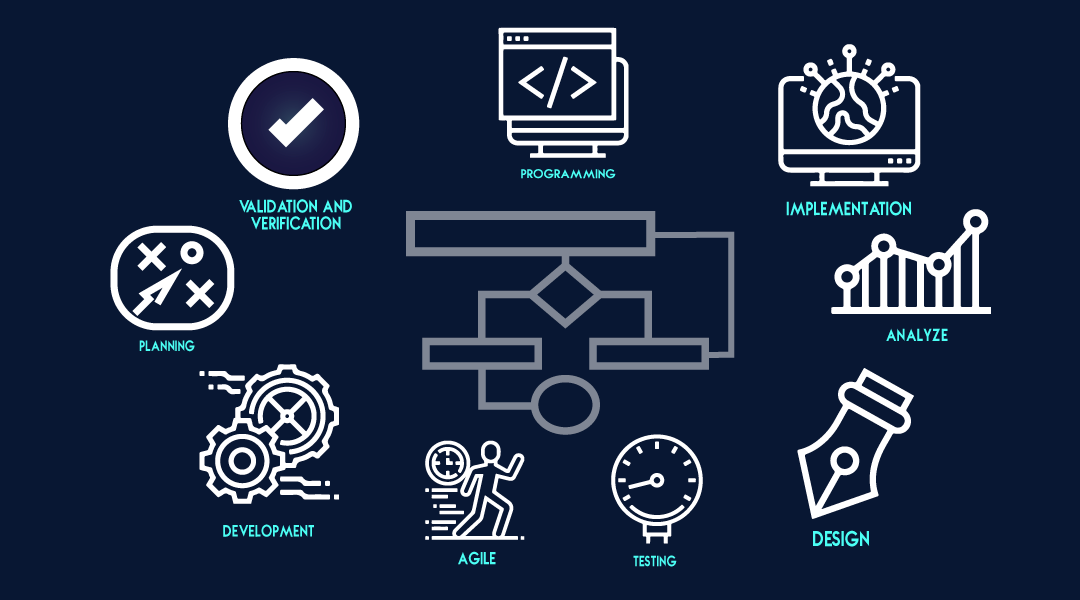
\includegraphics[scale=0.25]{Metodos.png}
\caption{Métodos de Planejamentos  de Engenharia de Software}
\citep{FotoAgeis}
\label{fig:universe}
\end{figure}                                %//Declaração da figura
%// lista

\section{Relevância da engenharia de software e sistemas}

A engenharia de software é importante para o futuro da humanidade, pois sua existência possibilidade a criação de sistemas mais avançados em níveis de complexidade.
O risco de atraso contido no desenvolvimento de uma aplicação, daí vem um dos focos dessa disciplina, buscando diferentes métodos e tecnologias para uma finalização
de projeto com menos surpresas indesejadas.
\citep{Sommerville}

\section{Relação com outras disciplinas}
    \subsection{Algorítimos e Estruturas de Dados}
    Nesta cadeira  é requisitado a construção de algoritmos\\ de níveis mais avançados. Tornando assim a engenharia\\ de software
        uma matéria destaque para o melhor\\ entendimento do assunto de forma geral. 
    \subsection{Tópicos Avançados em Engenharia de Software}
    Nesta cadeira  é vista 
       de forma mais ampla\\ e conceitos mais aprofundados da engenharia\\ da software.


\bibliographystyle{plain}
\bibliography{wbh}
\end{document}
                                            %//achar o bibtex do artigo para fazer a referencia